\begin{appendices}

\addtocontents{toc}{\protect\setcounter{tocdepth}{1}}
\label{app_questionnaire}
\chapter{Data Collection of the User Study}
This chapter presents the questionnaires provided for each participant in the study.
Not all questions were shown for the human trainer group in \textit{Demographic Data} and \textit{Guided Interview} because these were specifically related to the interactive system group.
Each questionnaire is accommodated in separate sections.
Participants fulfilled the questionnaires as structured in the following order.

\clearpage

\section{Demographic Data}
\begin{figure}[htb]
	\centering
	\begin{minipage}[t]{0.82\linewidth}
		\centering
		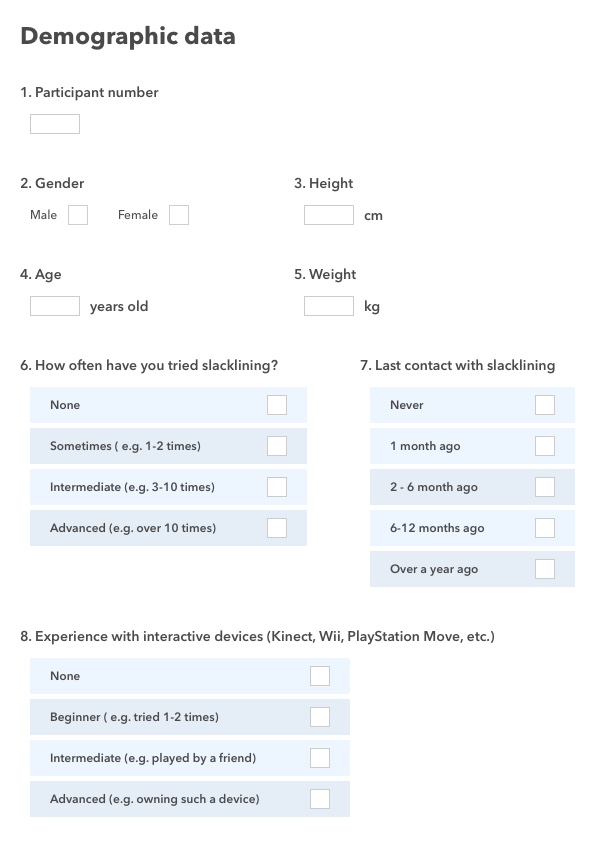
\includegraphics[width=1\linewidth]{Pictures/App_DemographicDataISG}
		\caption{Demographic data for participants in the study. Question 8 was just shown for the interactive system group}
		\label{fig:App_DemographicDataHTG}
	\end{minipage}
\end{figure}

\clearpage

\section{Physical Activity Questionnaire}
\begin{figure}[htb]
	\centering
	\begin{minipage}[t]{0.82\linewidth}
		\centering
		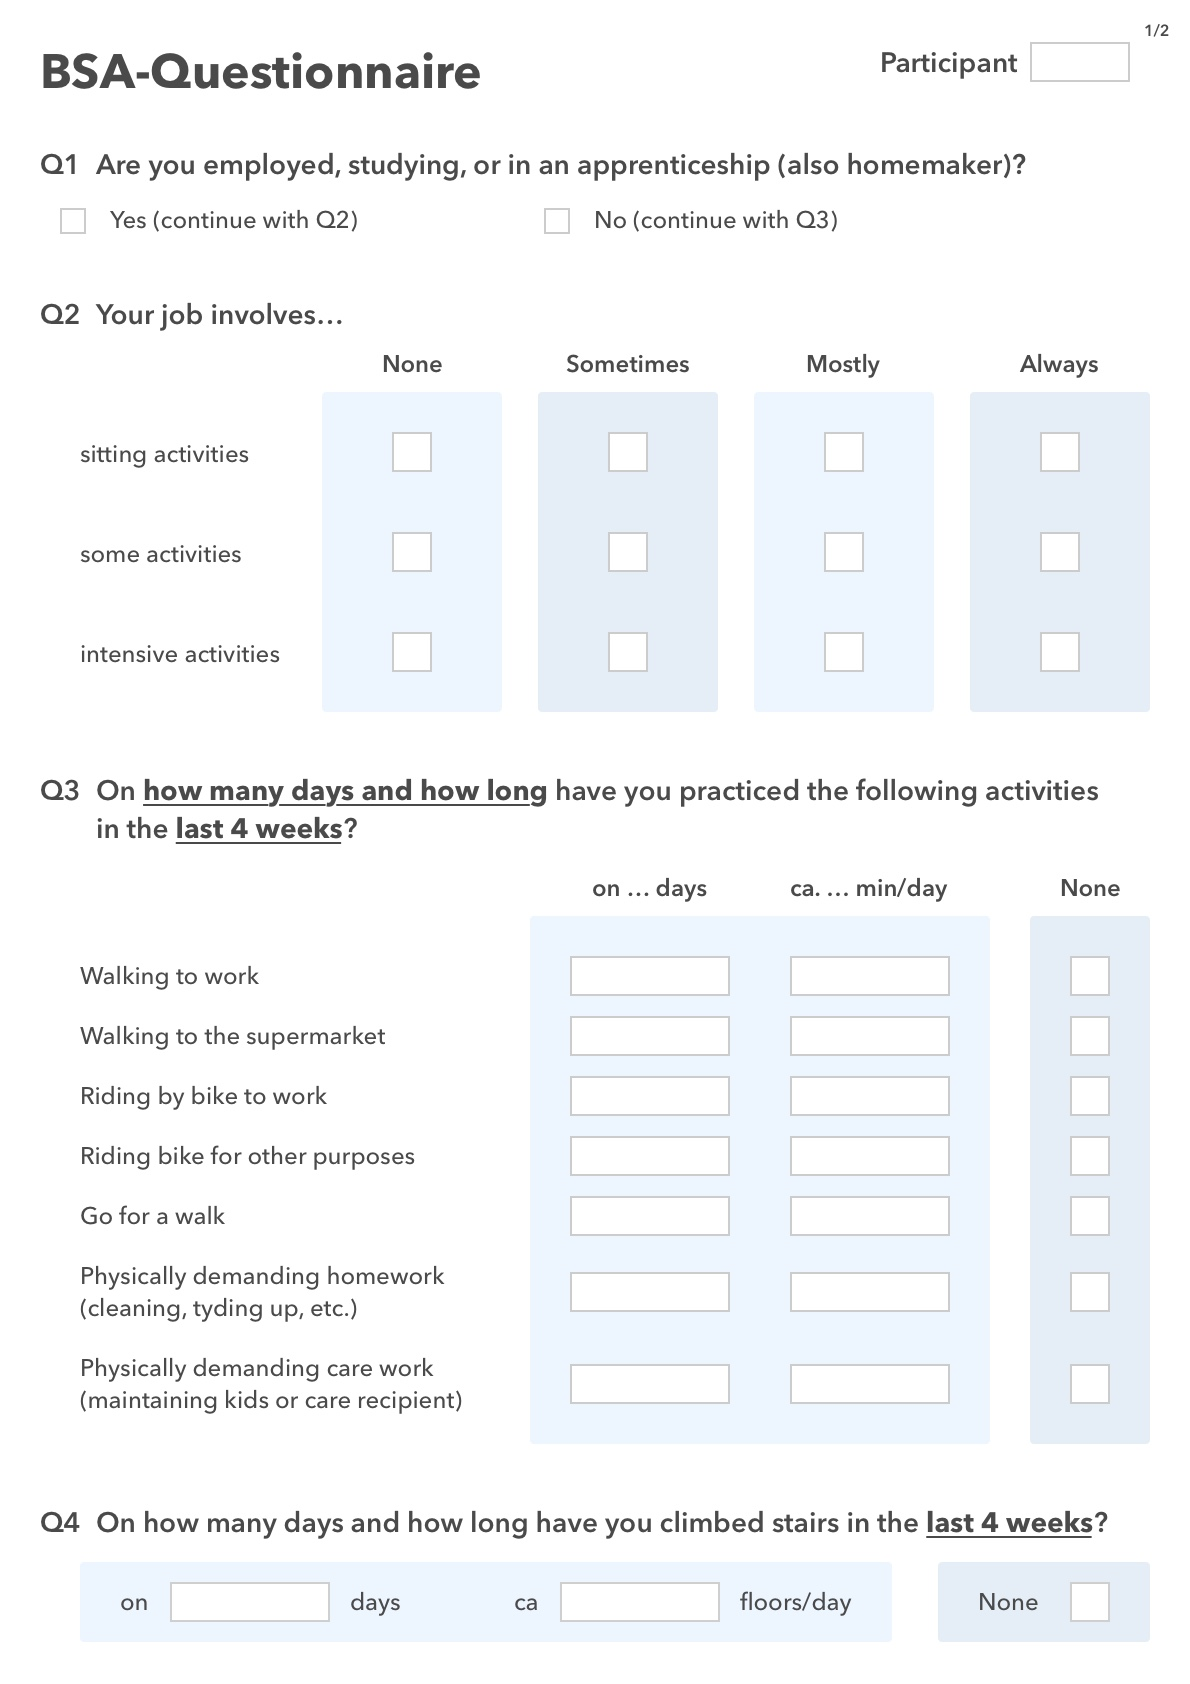
\includegraphics[width=1\linewidth]{Pictures/App_BSA1}
		\caption{First page of the physical activity questionnaire, adapted from Fuchs et. al~\cite{Fuchs2015-bsa}}
		\label{fig:App_DemographicDataHTG}
	\end{minipage}
\end{figure}

\begin{figure}[htb]
	\centering
	\begin{minipage}[t]{0.82\linewidth}
		\centering
		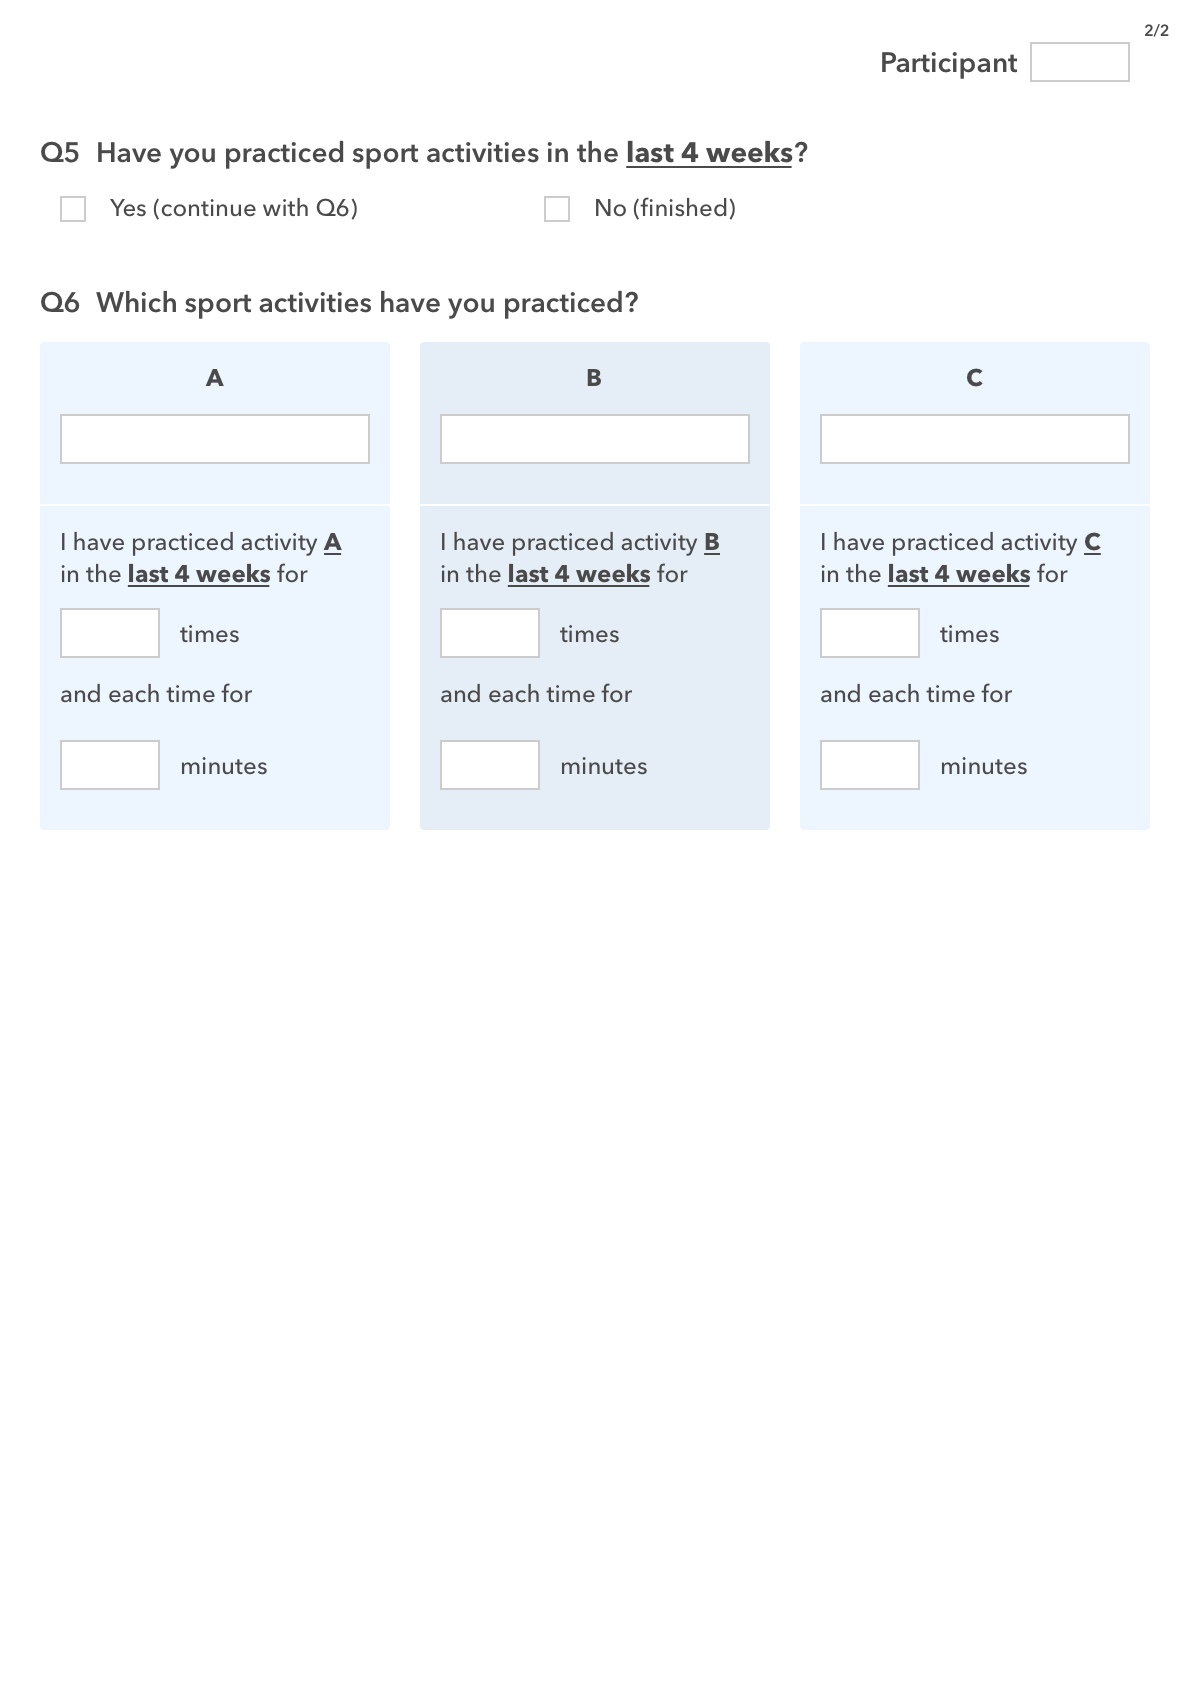
\includegraphics[width=1\linewidth]{Pictures/App_BSA2}
		\caption{Second page of the physical activity questionnaire, adapted from Fuchs et. al~\cite{Fuchs2015-bsa}}
		\label{fig:App_DemographicDataHTG}
	\end{minipage}
\end{figure}

\clearpage

\section{Lateral Preference Inventory}
\begin{figure}[htb]
	\centering
	\begin{minipage}[t]{0.82\linewidth}
		\centering
		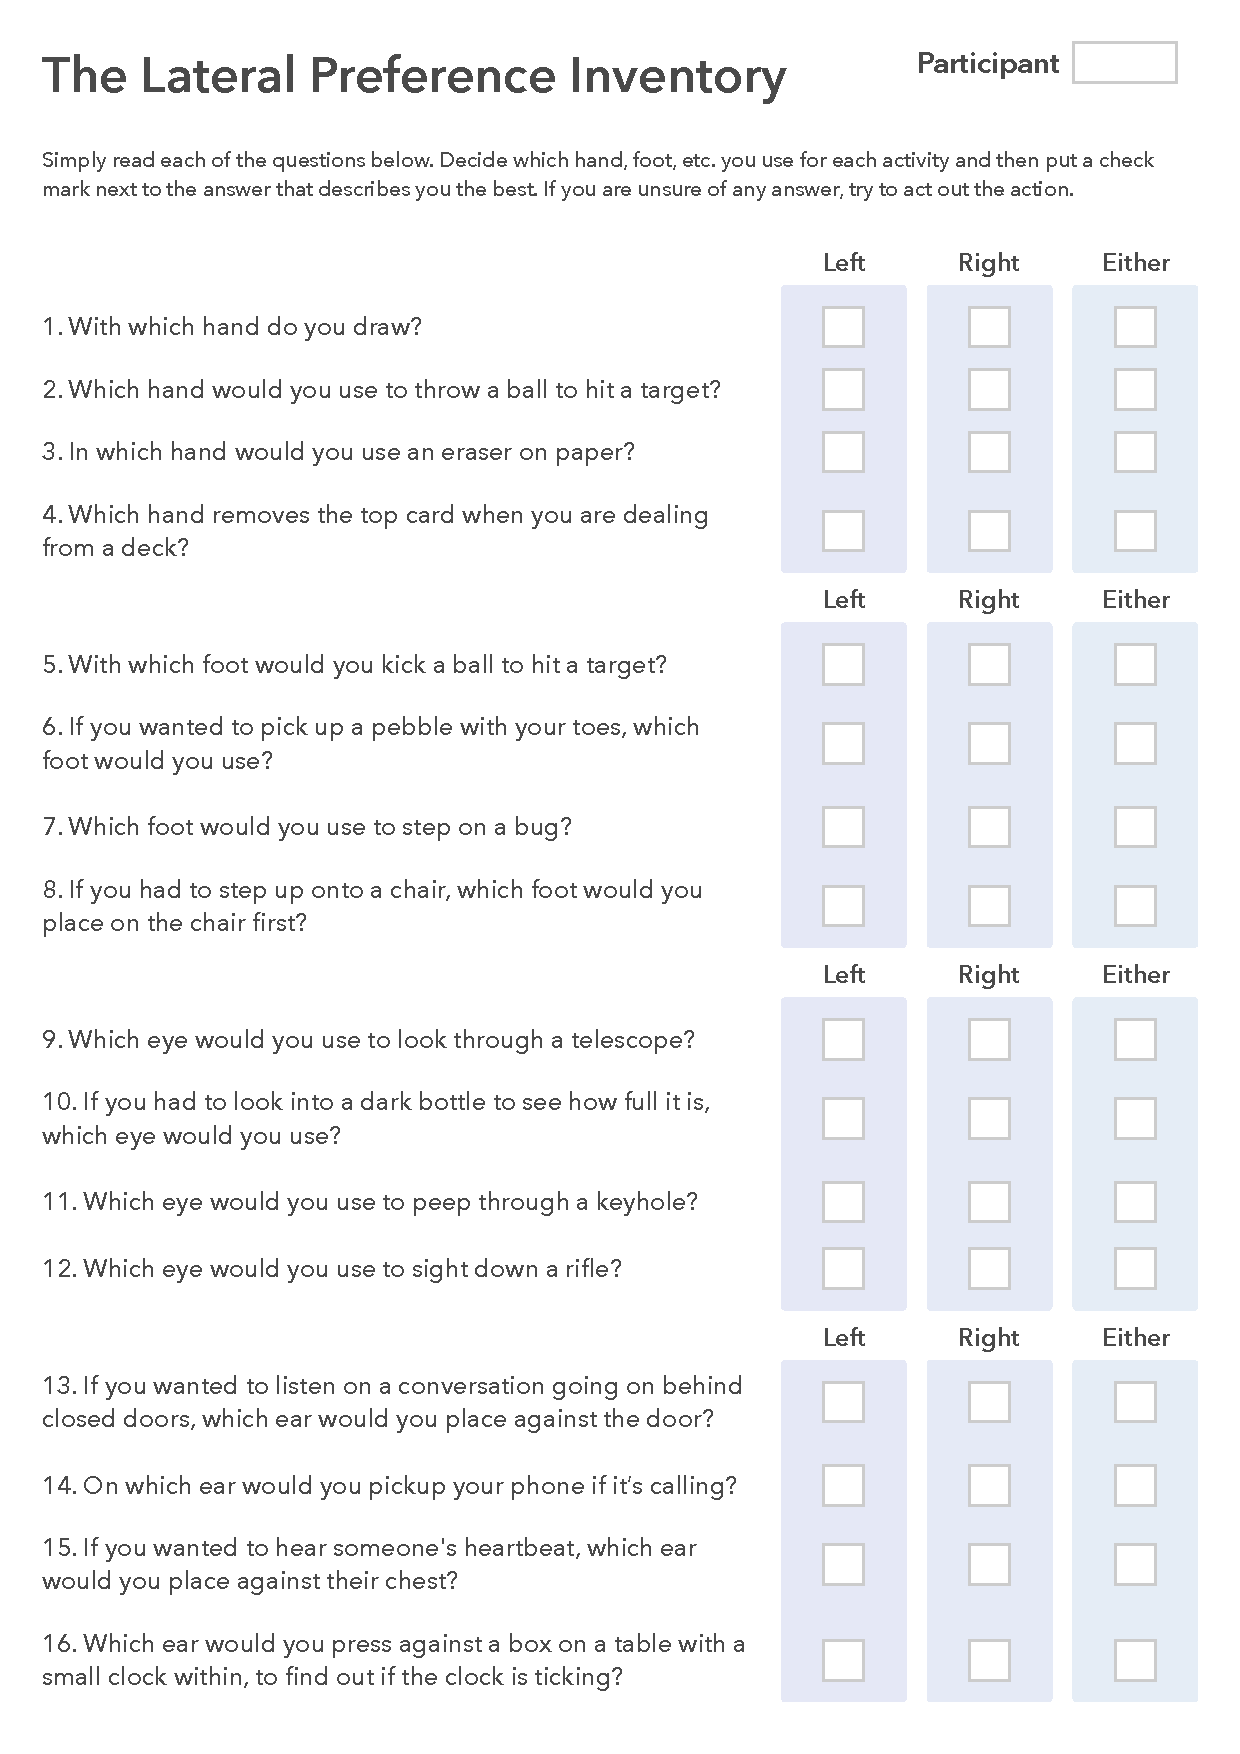
\includegraphics[width=1\linewidth]{Pictures/App_LateralPreference}
		\caption{Lateral preference inventory to determine the preference of the body side, adapted from Coren~\cite{Coren1993-lp}}
		\label{fig:App_DemographicDataHTG}
	\end{minipage}
\end{figure}

\clearpage

\section{Guided Interview Questionnaire}

\subsection*{Block 1: General questions about the learning method}
Q1: How is your general experience about this training method?

Q2: What do you like the least?

Q3: What do you like the most?

Q4: Would you use this method and why?\\

\subsection*{Block 2: Application scenarios}
Q1: Could you think of any other application scenario for exactly this training method with the slacklining approach? (no hints but e.g. rehabilitation, sport medicine, etc.)

Q2: Could you think of any other sport activities, than slacklining, that could fit in this method?\\

\subsection*{Block 3: User Interface / System Feedback Evaluation~\footnote{These questions were just asked for the interactive system group}}
Q1: What do you like the most about the system?

Q2: What was most frustrating / disturbed you?

Q3: What would you change?

Q4: How would you describe the system in one sentence?

\chapter{Statement of the Ethical Review Board}
\begin{figure}[htb]
	\centering
	\begin{minipage}[t]{0.62\linewidth}
		\centering
		
\includegraphics[width=1\linewidth]{Pictures/App_EthicalReviewFeedback}
		\caption{Approvement of the Ethical Review Board in response to the research project}
		\label{fig:App_DemographicDataHTG}
	\end{minipage}
\end{figure}
\end{appendices}
